\documentclass[11pt]{article}
\usepackage{amsmath}
\usepackage{graphicx}
\oddsidemargin 1mm

\textwidth 6.3in 
\topmargin -5mm
\headheight 5mm 
\headsep 8mm
\textheight 8.9in

\renewcommand{\floatpagefraction}{.8}
\renewcommand{\baselinestretch}{1.0}
\parindent 0pt
\parskip  4pt

%%=========================================================
\begin{document}
\noindent
\thispagestyle{empty}
\sloppy

\rule{1mm}{0mm}

\vspace{-17mm}
{\LARGE \bf Midlevel Prosodic Features Toolkit }

\smallskip
{\large \bf incorporating the  Prosody Principal Components Analysis Workflow}
\medskip


{\LARGE \bf Version 7.3}
\vspace{7mm}


{\bf Nigel Ward, University of Texas at El Paso}

{\bf \today }

\vspace{-1ex}

\begin{tabular}{p{7cm}rl}
  & \ref{sec:overview} & Overview  \\
  & \ref{sec:starting} & Getting Started \\
  & \ref{sec:blackbox} & Using it as a Black Box, for Pattern Discovery \\
  & \ref{sec:pca-overview} & PCA-based Analysis Overview \\
  & \ref{sec:file-formats} & File Formats \\
  & \ref{sec:interpreting}  & Interpreting the Dimensions \\
  & \ref{sec:subpopulations}  & Comparing Populations \\
  & \ref{sec:features} & Feature Computations\\ 
  & \ref{sec:pitch} & Pitch Trackers \\ 
  & \ref{sec:robustness} & Robustness \\
  & \ref{sec:validation} & Validation \\
  & \ref{sec:history} & History \\
  & \ref{sec:future} & Future Work \\
  & \ref{sec:location} & Availability and Location Notes
\end{tabular}

\vspace{-3.5ex}
%%=========================================================
\section{Overview}    \label{sec:overview}

This toolkit supports prosodic analysis of speech, especially dialog,
and especially statistical and machine-learning work.
This may be useful for you:
\begin{itemize}\setlength{\itemsep}{0pt}\setlength{\parskip}{0pt}
\item as a source of code to compute individual
prosodic features 
\item for producing a full set of prosodic features
suitable as input to machine-learning algorithms 
\item as a complete
workflow for discovering patterns of prosodic or multimodal behavior.
\end{itemize}
It contains a novel set of prosodic features that are robust,
everywhere-computable, fairly comprehensive, reasonably fast, and
proxy for several perceptual qualities.  In this it has some
advantages over more commonly used packages such as OpenSmile,
Covarep, Voicebox, Praat, and Novoic's Surfboard. It also contains a
workflow for analysis including Principal Components Analysis (PCA)
and various support for automated and human-in-the-loop analyses.

This document assumes a basic familiarity with prosody and its
acoustic measures, as obtainable, for example, from \cite{me-cup},
Chapter 4 of \cite{ogden-phonetics} or Chapter 4 of
\cite{ladefoged03}.

This document is a work in progress.  Comments and suggestions are
welcome.


%==========================================================
\section{Getting Started}  \label{sec:starting}

The code is at {\tt https://github.com/nigelgward/midlevel }.  It requires
%\begin{itemize}\setlength{\itemsep}{0pt}\setlength{\parskip}{0pt}
 Matlab. (This was developed mostly on release r2015a, but seems to
 work on some earlier releases and forward through r2019a.  r2020
 apparently renamed the function {\tt hanning} to {\tt hann} and moved
 it to the Signal Processing Toolkit, so if that causes problems, it
 may be enough to just edit {\tt fxrapt.m} to rename {\tt hanning} to
 {\tt hann}.)

% from voicebox: readau, voicebox, fxrapt, winenvar,
%rfft, irfft, v_findpeaks, lpcauto, distitar,
% lpcar2ra, lpcar2rr, lpcar2rf, lpcrf2rr

For an initial test of whether it runs for you, download the code,
enter Matlab, do {\tt addpath} for {\tt midlevel/src}, {\tt
  midlevel/src/voicebox}, and {\tt midlevel/flowtest}, then {\tt cd}
to the {\tt flowtest} subdirectory, and do {\tt
  findDimensions('.', 'minicrunch.fss');}. In a minute or
so this should create a {\tt loadings.txt} file; if so, the code is
probably working fine.

If you are interested only in using the features, skip ahead to read
Section \ref{sec:features}, and then back to Section
\ref{sec:file-formats} for the file formats.

In general, to prepare to work on your own data, you'll need to do
three things: 1) convert it to the right format, 2) create an
inventory of audio files to process, and 3) select a feature set to
use, as described in Section \ref{sec:file-formats}.


%===========================================================
\section{Using it as a Black Box, for Pattern Discovery} \label{sec:blackbox}

If your aim is simply to derive insight on the prosodic constructions
of a language or dataset:

\begin{itemize}   \setlength{\itemsep}{0pt}\setlength{\parskip}{0pt}
\item download this toolkit to a directory called {\tt midlevel} somewhere 
\item start up Matlab
\item {\tt addpath} for three directories: {\tt midlevel/src}, {\tt
  midlevel/src/voicebox}, and {\tt midlevel/src/voicebox}, with the
  exact directory names depending on your download destination
\item {\tt cd} to the directory containing your audio files
\item {\tt c2c();}
\item examine the loadings, as seen in the figures in the {\tt
  loadingplots} directory
\item listen to timepoints in your data where a dimension has extreme
  high or low values, as listed in the files in the {\tt extremes}
  directory
\end{itemize}


%==========================================================
\section{PCA-Based Analysis Overview }   \label{sec:pca-overview}

This toolkit was designed to apply Principal Components Analysis over
prosodic feature collections computed over dialog datasets of an hour
or so.  This is useful, we have found, for various purposes.  It gives
dimensions which correspond to interpretable patterns of behavior
\cite{prosodic-elements}.  The values of these dimensions usefully
characterize the instantaneous state of the dialog
\cite{dialog-dimensions}.  Applications so far include language
modeling, information retrieval, filtering, gaze prediction, finding
patterns of action-coordinating prosody, distributional analysis,
predicting actions from prosody, and examining non-native dialog
patterns
\cite{pca-lm,prosody-ir,sigdial-codec,ward-gaze,ward-abu,dimensions-uh-huh,l2english,me-mandarin,ward-stance}.
Before reading further you may want to read one of these papers for an
overview of the approach and the features.

There are two main use cases, related as seen in Figure \ref{diagram},
and described in the following subsections.

\begin{figure*}[thp]
 \centerline{ 
 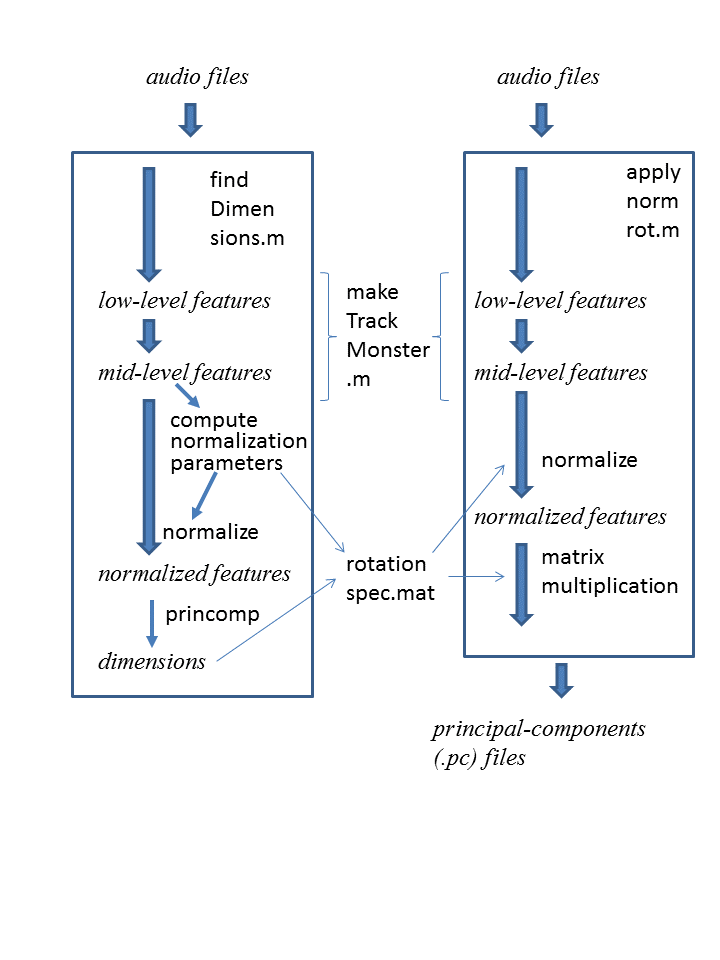
\includegraphics[width=11.4cm, trim = 0.cm 4.3cm 0cm 1.5cm, clip=true]{workflow-overview}
}
\caption{Workflow Overview}
\label{diagram}
\end{figure*}


%-------------------------------------------------------
\subsection{Apply Rotation}    \label{applynormrot}
 
This computes, for each moment of a dialog, the values of the
principal components at that moment.  For most purposes this will be
done using some standard, pre-computed principal components, together
with some standard normalization parameters.  (The results may make
more sense if the file to be processed is from the same set as the
audio used to generate the normalization parameters (Section
\ref{computerotation}), to avoid potential problems due to
different domains, speaking styles, or languages.  Recording
conditions may also be an issue, although the features are designed to
be fairly robust to these.)

Thus the function {\tt applynormrot.m} creates a {\tt .pc} file for
each track of one or more audio files; it does this in five steps:
\begin{itemize}   \setlength{\itemsep}{0pt}\setlength{\parskip}{0pt}
\item read in an audio file or set of files
\item compute the raw  features
\item normalize them, using  precomputed parameters (means and
  standard deviations)
\item  rotate them, using a precomputed rotation
\item write the results to {\tt .pc} files, and also locations of dimension
  extremes.
\end{itemize}

The resulting dimension-based representation can then be as input to
for various tasks, or can be interpreted, as described in Section
\ref{sec:interpreting}.

%$\clubsuit$ every invocation of findDimensions.m or applynormrot.m,
%should be documented in and automatically-created logfile, including
%timing information, written to the same directory the .pc files are
%in, as additional provenance beyond the on-line header.

%------------------------------------------------------------------
\subsection{Compute Rotation} \label{computerotation}

In order to do the above, there of course needs to be a
normalization-and-rotation available to work with.  {\tt
  findDimensions.m} creates this.  The steps it performs are:
\begin{itemize}   \setlength{\itemsep}{0pt}\setlength{\parskip}{0pt}
\item read in an audio file or files
\item compute the raw  features
\item compute normalization params, then use them to normalize the features
\item compute the rotation, that is, do PCA to discover the dimensions
\item save the rotation coeffs and the normalization params for later use (Section \ref{applynormrot})
\end{itemize}

The PCA itself is done using Matlab's {\tt princomp} function.  This
is memory-intensive.  If you're processing a lot of audio (more than,
say, 100 minutes), then first compute the rotation using just a
subset, then apply it to everything.  If this is not done, Matlab
will gobble memory and freeze or crash the machine.


%------------------------------------------------------------------
\subsection{Overview of the Arguments}   \label{arguments}

In general,  five things are  needed to completely specify either
of the above processes.  Three of these are arguments

\begin{description}  \setlength{\itemsep}{0pt}\setlength{\parskip}{0pt}
\item[tracklist] specifies which tracks to process, each being a
  track from an audio file (Section \ref{tracklist-files})
\item[featurespec file]  specifies the set of features to use (Section \ref{featurespec-files})
\item[output dir] specifies where to write the resulting {\tt .pc}
  files (one per track), and extremes files (one per dimension)
\end{description}

and two  are locations which are set implicitly:

\begin{description}  \setlength{\itemsep}{0pt}\setlength{\parskip}{0pt}
\item[pitch cache] is the subdirectory where to store (or find) the f0
  values as computed by {\tt fxrapt}, as {\tt .mat} files.  This
  subdirectory is created in the same directory where the audio files
  are located, as specified in the tracklist file.
\item[parameter dir] is the directory where to store (or find) the
  params and coeffs (notably in the file {\tt rotationspec.mat}), and
  the various human-readable files, notably the logfile, correlation
  coefficients, and factor loadings.  This directory is implicitly set
  to be the location where the matlab process is run.
\end{description}

Given the implicit storing of the params and coeffs, it's probably
best to create a new directory for each project.  If all relevant
Matlab work is done in this directory, then all the parameter files
will be written here and then found again without difficulty.


%%=========================================================
\section{File Formats}        \label{sec:file-formats}

%--------------------------------
\subsection{Data Files}

First there are the data files, each representing an audio track or
file, at various stages of processing.

\begin{description}   \setlength{\itemsep}{0pt}\setlength{\parskip}{0pt}

\item [---.au] The input.  An audio file, 16 bit, linear PCM, 8K
  sampling, of no more than 10 minutes.  While sometimes longer files,
  other {\tt .au} formats, and even {\tt .wav} files, often work fine,
  it is safer to use this format. The {\tt sox} program is convenient
  for conversions to this format.  The workflow was originally
  designed to handle stereo recordings, with each speaker in a
  separate track, but monoaural data can also be handled.  If an mono
  {\tt .fss} file (see below) is used.

\item[---f0.mat] a file specifying for an audio track the pitch every
  10 milliseconds.  These files are created because {\tt fxrapt} is
  time-consuming, so it's worth caching the results to avoid
  recomputing them.

\item[---.pc] The output: a principal components file.  There is a
  one-line header describing the provenance.  Each subsequent line
  describes the prosody at one timepoint.  These are 10ms apart.  Each
  line contains a whitespace-separated list of, first the timepoint,
  then the values for all the principal components (PCs).  PCs appear
  in order of the variance explained.  These files are large and
  writing them takes a long time, so this function is usually
  commented out.
\end{description}


%%=========================================================
\subsection{Tracklist Files}       \label{tracklist-files}

This specifies the audio tracks to process.  The first line is the
directory in which the audio files are located.  Subsequent lines
specify the track and the file.  For example the line

\begin{quote}
\verb+l sw02079.au+
\end{quote}

means to process the left track of the specified Switchboard audio
file.  Tracklist files have the extension {\tt .tl}. 


%%=========================================================
\subsection{Feature Specification Files}     \label{featurespec-files}

To encode contextual information we need to use features computed at
various temporal offsets, relative to the point of interest.

As a default this point of interest is stepped through the audio,
every 10 milliseconds.  A ``featureset specification'' ({\tt .fss})
file specifies which features to use.  These thus describe how to
``crunch'' together data from individual computations into a single
composite matrix suitable for machine learning or dimensionality
reduction.

Many {\tt .fss} files exist, each designed for a specific purpose.
{\tt april.fss}, has more features for the primary-track talker than
for the other talker, so can be used to analyze one speaker's
behavior.  {\tt medslim.fss} has features evenly distributed across
the two speakers.  {\tt mono4.fss} is useful for information retrieval
in broadcast news.  {\tt minicrunch.fss} is a small set for testing
the workflow

In a {\tt .fss} file each line specifies a feature, window start,
window end, and the channel, for example

\begin{quote}{\tt 
    vo   -200   -100 self  \\
    cr    400    600 inte
}\end{quote}

where the first line means the speaker's average intensity (volume)
over a 100ms window that starts 200ms before the point of interest,
and the second line the interlocutor's average creakiness over a 200ms
window that starts 400ms after the point of interest.  ``Self'' refers
to the primary track, ``inte'' to the other track, containing the
interlocutor's voice.  The primary track is specified in the tracklist
file, as either left ({\tt l}) or right ({\tt r}).  If a fss file has only self
features (no ``inte'' features) it can be applied to mono files.


In fss files currently the following codes are recognized:


\begin{tabular}{ll}
  vo  & intensity (volume) \\
  vf  & voicing fraction \\
  sf  & speaking fraction \\
  sr  & speaking-rate proxy (also reflects enunciated vs.~reduced, and creaky vs.~modal) \\
  cr  & creakiness \\
\end{tabular}

\begin{tabular}{ll}
  fp  & flat pitch: degree of flatness \\
  np  & narrow pitch range: degree of narrowness \\
  tp  & typical pitch range (not often used)\\
  wp  & wide pitch range  \\
  hp  & high pitch (obsolete) \\ 
  lp  & low pitch (obsolete) \\
  th  & true high pitch: degree of highness  \\ 
  tl  & true low pitch: degree of lowness \\
\end{tabular}

\begin{tabular}{ll}
  pd  & late (delayed) pitch peak \\
  le  & lengthening, of a vowel etc. \\
  en  & enunciation (articulatory precision) \\
  re  & phonetic reduction \\
  vr & voiced-unvoiced intensity ratio \\
\end{tabular}

\begin{tabular}{ll}
  ts  & time since start of the recording (window start/end times ignored) \\
  te  & time until end of the recording (ditto) \\
  ns  & nearness to start of the recording (ditto) \\
  ne  & nearness to end of the recording (ditto) \\
\end{tabular}

\begin{tabular}{ll}  
  cp  & smoothed cepstral peak prominence, representing breathiness, etc. \\
\end{tabular}


Reserved two-letter code (implementation pending): 

\begin{tabular}{ll}  
  ha  & harmonicity \\
  br  & breathiness
\end{tabular}

Adding a new prosodic feature requires changing three things.  First
you create an entry for your new feature in the featurespec file,
choosing any unused two-letter code and an appropriate window size and
offset.  Second, you write a new matlab function to compute that
feature.  This might compute it from the audio, or from multimodal
data, or it might read values from a file that was written by an
external program.  Third, you add a new case to the big {\tt switch}
statement in {\tt makeTrackMonster} to associate your new
feature-computing function with the two-letter code.

Every feature-computing function is responsible for returning a vector
of values for windows centered every 10 milliseconds throughout the
audio file.  The first one is centered at 10 ms.  This is true for
both the frame-level features (energy and pitch) and for the derived
(mid-level) features, which span longer windows.  

All feature-computing functions must return values everywhere, even at
the start and end of the audio file.  In particular, while raw pitch
features can include NaNs, the mid-level features must be designed not
to. Mid-level features with windows longer than 10ms, when computed at
timepoints close to the start or end of a file, will stretch out
beyond the point of no data, and thus they will lack enough
information to return a fully meaningful value.  In such cases the
function should return an non-obtrusive value in the typical range
(rather than some extreme value like -9999, since that would mess up
the normalization).  While such values can be problematic, this is not
usually a problem, since the audio files we work with are usually long
enough (generally 2--10 minutes long) that the vast majority of
features values will be valid.


%%=========================================================
\subsection{Normalization and Rotation Parameter File}

{\tt rotationspec.mat}  contains the information pertaining to a
rotation.  This enables the application of an pre-determined rotation 
to new files.  It contains 

\begin{itemize}  \setlength{\itemsep}{0pt}\setlength{\parskip}{0pt}
\item the normalization parameters, namely for each feature its mean
  and its standard deviation

\item the PCA coefficients
\end{itemize}

A related file is {\tt loadings.txt}, which is a human-readable
version of the PCA coefficients.


%=======================================================
\section{Interpreting the Dimensions}  \label{sec:interpreting}

An important reason to use Principal Components Analysis is to
understand what's going on in the data.  For all data sets tried so
far, the dimensions output by PCA have turned out to be readily
interpretable as meaningful patterns of behavior.  

One preliminary is
to look at the variance and cumulative variance explained by the
PCA-found dimensions, which is written to {\tt variance.txt} by
findDimensions. 

Then there are three techniques to help you arrive at
interpretations:


%---------------------------------
\subsection{Examine the Factor Loadings}

{\tt findDimensions.m} includes a call to {\tt writeloadings.m}, which
writes a large, human-readable file called {\tt
  loadings.txt}.  While these files are readable, it's generally better
to visualize the loadings.  This can be done with:

\begin{verbatim}
   diagramDimensions('rotationspec.mat', 'xxx.fss');
\end{verbatim}

Where {\tt xxx.fss} is the name of the feature file used to create the
rotationspec.  This second parameter is optional unless you're using
an rotationspec that was written by a very early version of
{\tt findDimensions}.

This creates a {\tt loadingplots} directory and writes a diagram
per dimension as a {\tt .png} file.

%---------------------------------
\subsection{Listen to Extreme Examples}

To understand a dimension, it helps to listen to locations in data
where each dimension has extreme (the highest and lowest) values.  To
support this, the files {\tt dim00.txt} etc.\ are written in the {\tt
  extremes} subdirectory of outdir by {\tt findExtremes.m} (called by
{\tt applynormrot.m}, as described in Section \ref{applynormrot}).
This finds the extreme points in each file, but winnows out points too
close to each other, to provide some diversity.

Once we have these timepoints, it's time to listen.  There are lots of
tools that can do this.  One option is ``Didi''
(http://www.cs.utep.edu/nigel/didi/), which conveniently lets you jump
to 5 seconds before a desired timepoint, and then play this region,
and is conveniently invokable from the command line.  However Didi
only installs easily on 32-bit linux machines with Centos/Redhat 5.
Elan and VLC are also good choices.


%---------------------------------
\subsection{Consider Co-occurring words} 

The last source of insight for interpreting the dimensions is to see
find which words co-occur with values high/low on each dimension.
However this is only possible if we have transcribed data, and even
then, since the file formats vary, it requires custom code for each
case.


%=======================================================
\section{Comparing Populations}    \label{sec:subpopulations}

Different populations may use prosody in different ways.  Examining
their behavior with respect to the dimensions may be informative.  One
way is to examine basic statistics in how the distributions on the
dimensions differ.  (While helpful, this certainly does not give the
whole picture \cite{l2english}.)

These can be seen in {\tt summary-stats.txt}, which is written by {\tt
  applynormrot.m}.  Useful may be the average value (to detect bias to
one side of the dimensions), the standard deviation (to detect failure
to use a dimension much), etc.

Another way is to create histograms showing the distributions of two
populations, on the various dimensions, and eyeball them.  For example:

\begin{verbatim}
refvals = applynormrot('reference.tl', 'someset.fss', '/tmp');
newvals = applynormrot('new.tl', 'someset.fss','/tmp');
histograms(refvals, newvals);
\end{verbatim}


% There is also fragments of a workflow described in {\tt
%histo/README.txt}: in short, this uses {\tt distDist.m}, {\tt
%bhatd.m}, and {\tt binProbs.m} to generate histograms for each
%dimension, including superimposed histograms for the two populations,
%and to compute the Bhattacharyya distance.


%%=========================================================
\section{Features}               \label{sec:features}

%--------------------------------------------
\subsection{Frame-Level Feature Computations}

Three frame-level (low-level) features are computed: pitch, energy,
and cepstrum.

The raw log-energy is simply

\begin{equation}
e_f^r = log \sqrt{(\frac{1}{160} \sum\limits_{i=f-80}^{f+79} s_i^2)}
\end{equation}

where $f$ is the frame center and $s$ is the signal, assuming the
sampling rate is 16000 per second and the frames are 10 milliseconds
long.  This is computed in {\tt computeLogEnergy.m}.

The  raw pitch,
\begin{equation}
   p^r_f
\end{equation}


is obtained with {\tt lookupOrComputePitch.m}, which is a wrapper for
various functions as described in the next section.  This returns
values in hertz, or NaNs if there is no detectable pitch.

The cepstrum is computed using {\tt mfcc.m}.

Other frame-level features may later be added.  For example this might
include spectral features or features generated by {\tt Praat}
(notably NHR).

Frame-level features will include multimodal features, if so specified
in the {\tt .fss} file.  If keystrokes are specified, {\tt
  featurizeKeystrokes.m} is called to load that information; similarly
{\tt featurizeGaze.m} is called if gaze features are specified.

%--------------------------------------------
\subsection{Frame-Level Feature  Normalization}

Pitch is converted from hertz to percentiles, to normalize for
individual differences in pitch height and in pitch range.

\begin{equation}
p_f^p = percentile(p_f^r)
\end{equation}

where the percentile is based on the distribution of pitch values in
all voiced regions in the entire track.  These are mapped to the range
0 to 1; thus the lowest pitch value in the track maps to 0.0, the
highest to 1.0, and the median pitch value to 0.5.  As described
below, percentilized pitch is used for the highness and lowless
features; but raw pitch is used for the for creaky, wide and narrow
features.

Energy is normalized as described below. (It is not done at the frame
level, but over larger windows, because  frame-level
energy may be less clearly bimodal.)


%--------------------------------------------
\subsection{Mid-Level Feature Computation}   \label{other-features}

The mid-level features are as listed in Section
\ref{featurespec-files}.  Each summarizes something about the values
of the frame-level features across some window.  The motivations for
choosing these specific features and these specific implementations
are given in Chapter 9 of \cite{me-cup}.  There are many desiderata
for feature sets, some in conflict.  For this feature set, the primary
considerations were that it be everywhere-defined, robust, and simple.
Other considerations were that they be useful, have at least some
perceptual validity, and are reasonably fast to compute.  All of these
were explored spottily, not systematically.  Compatibility with
previous definitions or implementations was not a priority.

Each value is associated with the time at the center of the window.
Windows are shifted (stepped) every 10ms, because it's unlikely that
prosodic features change faster than that.  Typically these are
downsampled before use in applications.

These are intended to extract essentially all the useful information
in the frame-level features; for machine-learning applications, the
mid-level features should be the ones to use. 


%----------------------
\subsubsection{Window Energy}

We scale the energy to normalize for individual differences and
recording-condition differences, specifically regarding typical
speaking volume and noise floor.  To do this we find typical-silence
and typical-speech values of energy, using {\tt findClusterMeans.m}.
This implements a simplified 1-dimensional k-means algorithm ($k$=2)
and applies it to over all $e^r$ values in the track, using as seeds
the min and max of $e_f^r$ over the entire track.  We then normalize
the energy with respect to these values.

\begin{equation}
e_f = \frac{ e_f^r - e^{silence} }{e^{speech} - e ^{silence}}
\end{equation}

where $e^{silence}$ is the typical silence energy and $e^{speech}$ is
typical speech energy.  Thus the resulting $e$ is on a scale where
typical vowel volumes are 1 and typical silent frames are 0.

This is not the simplest way to normalize, but it seems suitable.
The average volume across a track will vary with the amount of
speaking the person in that track is doing.  Thus we want to ensure
that each person, when he is speaking, is reported has having the same
volume on average.  (Of course some people have quieter voices than
others, but we're only interested in whether a speaker is being quiet
or loud relative to his typical speaking volume.)  There may also be
slow variations in gain, if the talker varies the handset-to-mouth
distance, but these we don't deal with.

%----------------------
\subsubsection{Pitch Highness}

\begin{equation}
h_{a,b} = \frac{1}{b-a} \sum\limits_{i=a}^b (p_i^p -.5 | p_i^p> .5 \operatorname{and} p_i \neq NaN)
\end{equation}

where $a$ is the start of the window and $b$ is the end, both in
frames.  We use windows of various sizes, thus $a-b$ may be 5 (for a
50 milliseconds window), 10 (for a 10 ms window), etc.

Note that this computation uses the pitch
percentile values.



%--------------
\subsubsection{Pitch Lowness}

\begin{equation}
l_{a,b} = \frac{1}{b-a} \sum\limits_{i=a}^b ( .5 - p_i^p | p_i^p < .5 \operatorname{and} p_i \neq NaN)
\end{equation}

%--------------
\subsubsection{Creakiness}

\begin{multline}
c_{a,b} = \frac{1}{b-a} \sum\limits_{i=a}^b \enspace 1 \operatorname{if}  .475 < \frac{p_i}{p_{i+1}} < .525 \operatorname{or} \\  .80 < \frac{p_i}{ p_{i+1}} < .95  \operatorname{or} \\ 1.05 < \frac{p_i}{ p_{i+1}} < 1.25 \operatorname{or} \\ 1.90 < \frac{p_i}{ p_{i+1}} < 2.10
\end{multline}

Creak can be seen to affect computed $F_0$ in two main ways: the
presence of octave jumps and the presence of frame-to-frame pitch
jumps beyond what one would normally expect \cite{keating15}.

The thresholds are based roughly on what is known about maximum
human-achievable variation in pitch.  This is reported to be 61.3
semitones per second up and 70.6 semitones per second
down\cite{xu02-pitch-change-rate}.  Since a semitone is a 6\% rise or
fall, this means excursions greater than 3.6\% per frame up or
4.2\% per frame down are not normal pitch movements. 

Accordingly, in the equation the first clause detects pitch halving: a
pitch point within 5\% of half the value of a neighboring pitch point
counts as evidence for creaky voice.  Similarly the last clause
considers a pitch point that is within 5\% of twice the value of a
neighboring pitch point to also be evidence for doubling and thus
creaky voice.  The tolerance (5\%) is a little wider than Xu's results
would imply, mostly because pitch tracking of spontaneous speech is
not always highly accurate.

The second and third clauses detect variation in pitch that is too
large to be a normal pitch movement.  Again the 5\% criterion is used,
for the same reason.  

To explain this equation in another way, every pair of pitch points
counts as evidence for creaky voice except, a) those that are probably
due to normal pitch movements, with a ratio of between 0.95 and 1.05,
which are the vast majority, and b) those that are probably due to
noise of some kind, namely those with a ratio below .475 or above
2.10, or a ratio between 0.525 and 0.80, or a ratio between 1.25 and
1.90.  These specific thresholds are based purely on experience.

%--------------
\subsubsection{Narrowness}

\begin{equation}
n_{a,b} = \frac{1}{b-a} \sum\limits_{i=a}^b \sum\limits_{i-50}^{i+49} \enspace 1 \enspace \operatorname{if} 0.98 <  \frac{p_i}{p_{i-1}} < 1.02 
\end{equation}

where 50 refers to 50 frames.  With the nested {\em for} loop this is
somewhat inefficient, but this has not been a problem in practice.

This computation sums up the evidence for some narrow (flat) pitch
involving the window from $a$ to $b$.  While there are many ways in
which this could be done, this method was chosen in part because it is
robust to pitch halving and doubling, but mostly because it is simple.



% the normal declination across utterances ranges from 8 to 1
%semitones per second \cite{yuan-declination}.

%--------------
\subsubsection{Wideness}

\begin{equation}
w_{a,b} = \frac{1}{b-a} \sum\limits_{i=a}^b \sum\limits_{i-50}^{i+49} \enspace 1 \enspace \operatorname{if} 0.7 <  \frac{p_i}{p_{i-1}} < 0.9 \operatorname{or} 1.1 <  \frac{p_i}{p_{i-1}} < 1.3
\end{equation}

Note that if the ratio is more extreme, one of the two pitch points is
likely to be spurious, so we don't consider such cases to be evidence.


%--------------
\bigskip
\subsubsection{Window Energy:}

\begin{equation}
e^w = \frac{1}{b - a} \sum\limits_{i=a}^{b}e_i
\end{equation}

%--------------
\subsubsection{Energy Flux}
\begin{equation}
r = \frac{1}{b - a} \sum\limits_{i=a}^{b-1}|e_i - e_{i+1}|
\end{equation}

This was our first attempt at a proxy for rate.  It seems to correlate
also with the carefulness of articulation, and with creaky voice.

**** {\tt mrate}
(namely speaking rate, although in \cite{timelm} we found it worse
than amplitude variation (ampvar, sometimes also called jitter) as a
speaking-rate proxy).


%--------------
\subsubsection{Late Pitch Peak}

This is described in the comments in epeakness.m, ppeakness.m,
computeSlip.m, computeWindowedSlips.m, and laplacianOfGaussian.m. 

%-------------
\subsubsection{Lengthening}

This is described in lengthening.m, and also in doc/lengthening-rate.txt.

%-------------
\subsubsection{Enunciation and Reduction}

These are described in the comments of cepstralDistinctness.m.

%-------------
\subsubsection{Voiced-Unvoiced Intensity Ratio}

This is described in the comments of voicedUnvoicedIR.m.

%-------------
\subsubsection{Temporal Features}

The features {\tt ts}, {\tt te}, {\tt ns}, and {\tt nr} are computed
directly in makeTrackMonster.m

%--------------------------------------------
\subsection{Feature Assembly}

The relevant features at any point in time are not just those anchored
at that point, but also contextual features from the past or future,
and from the interlocutor as well as the speaker.  We therefore need
to assemble all these features.  Essentially this just requires
concatenating the various mid-level features, after each is shifted
(offset) appropriately.

The output is a huge monster array with {\it nfeatures} columns and
{\it ntimepoints} rows.

For some purposes these assembled features can be useful, as input to
various machine learning algorithms, without going on to the rotation
step.  To write data for such purposes, one can add a call to {\tt
  write\_pc\_file.m} on the monster array in {\tt makeTrackMonster}
etc. .


%--------------------------------------------
\subsection{Overall Normalization}

Before doing PCA we need to normalize the features to all have zero
mean across all dialogs in the training set.  (This is subsequent to
the frame-level pitch and energy normalizations described above.)
It's also helpful to normalize so that each feature has same standard
deviations, so that features with larger variance do not dominate.
(The mid-level features are far from normally distributed, and after
normalization that's still true, but this is probably only an
aesthetic problem.)

%log-pitch is approximately normal.  pitch height, being
%percentile-based, is flat in distribution, our pitch-height and
%pitch-range features are sparse, or, more correctly,  skewed, with lots
%of values near zero and a long tail.
%Energy is bimodal, with 0 being
%typical silence and 1 being typical speech.  ampvar is probably
%trimodal, with high values in consonant-dense regions, moderate values
%in vowels and slower regions, and small values in silence regions.  

Note that we do {\em not} normalize by file.  Any particular speaker
may have his own typical speaking style, different from others, and we
don't want to lose that information.  (When Shreyas tried normalizing,
file-by-file, to have each individual file have zero mean, all
language-modeling benefit was lost.)

%%=========================================================
\section{Pitch Trackers}   \label{sec:pitch}

At the root of many of the midlevel features is the frame-level pitch.
The toolkit supports two ways of computing this.  

The first is Mike Brookes's Voicebox function {\tt fxrapt.m}, which is
conveniently written in Matlab and very well documented.

The second is David Talkin's Reaper.  I added because it can handle
the Switchboard files that {\tt fxrapt} cannot.  (I'm guessing that
the problem is due to recording issues with some files, as discussed
in {\tt https://catalog.ldc.upenn.edu/docs/LDC97S62/swb1\_manual.txt}
in Section 13.)  Another advantage is that it is about 7 times faster.

(Other alternatives explored were Matlab's built-in pitch tracker,
which seems to have a lot of outliers and false alarms, and {\tt
  Yappt}, which also fails on many Switchboard files, including some
that {\tt fxrapt} could handle, and {\tt Praat}, which seems slow and
awkward for integrating.)

Reaper is in C++, and it runs only on {\it mono} files, so the
integration with the midlevel toolkit is awkward. The bash code {\tt
  reaperize.sh} does what's needed for processing Switchboard files,
and serves as an illustration of the necessary steps.

Since the midlevel features depend on the pitch detector, and were
tuned (somewhat) to work well with the quirks of {\tt fxrapt}, it's
worth noting that, on a tiny sample, {\tt reaper}'s output looked
visually smoother and more accurate than that of {\tt fxrapt}, which
likely  changes the behavior of the creaky voice feature.

Another issue is the question of whether to set the bounds differently
for male and female speakers.  This makes a huge difference for {\tt
  Praat}, but appears not to matter much at all for {\tt reaper}, so I
don't.


%%=========================================================
\section{Robustness}           \label{sec:robustness}

The toolkit is designed to be robust to normal human voice variation
and modest noise, but it is not robust to every form of
corruption. Files that contain splices mess up the default pitch
tracker, as noted above, and also the cepstrum computation.  The
symptom in both cases manifests as NaN values.  The easiest cure is to
exclude the offending file, e.g.\ English Callhome 4065, or to trim the
file to exclude the troublesome region, for example with {\tt sox
  bad.au cleaned.au fade 0 -1 0.01}, as for some Switchboard files.
Background music can also be a problem.


%%=========================================================
\section{Validation}   \label{sec:validation}

Testing for most of the feature computation methods was done using
both synthetic test data and small audio test files.  Details are
given in the comments of each Matlab file.  A small test harness is
included as {\tt validateFeature.m}.

To see the values of various low-level and mid-level features as they
vary over an audio file, uncomment the various {\tt plot} commands in
{\tt makeTrackMonster.m}.  One can then listen to the audio file,
using any available player, to see whether the feature values are
indeed high and low where they should be.

As an indirect check on correctness of the feature computation and
collating, one can examine the correlations among the features.  Every
call to {\tt findDimensions.m} creates a file, {\tt
  post-norm-corr.txt}, which lists, for each feature, the most highly
correlated and most anticorrelated other features.  (This is output by
{\tt output\_correlations.m}.)


%%=========================================================
\section{History}           \label{sec:history}

Version 1.  In our language  modeling work, we observed
problems due to the non-independence of our prosodic feature set.
Early in 2011 Olac Fuentes suggested we solve this by applying
principal components analysis.  In Summer of 2011 Justin McManus
prototyped the use of PCA on prosodic features for language modeling,
working with just four raw features.

Version 2. Starting Fall 2011, Alejandro Vega extended the code to
handle more features and made it work for features at different
offsets and over different window sizes.
%, and documented it in
%``Principal Component Analysis on Long Range Prosodic Features'',
%available locally at {\tt
%  /home/research/isg/speech/uteplm/documentation/howto.tex} and {\tt
%  /home/research/isg/speech/timelm/switchboardPCx/documentation/}.  He
%applied these to Switchboard data, probably the files listed in {\tt
%  fulltest/alex16.tl}.  (The audio files are on the CDs, but some
%other sample Switchboard files are in {\tt
%  /isg/speech/uteplm/switchboardau/}.)  The factor loadings this gave
%are in {\tt isg/speech/timelm/switchboardPCx/factorLoadings},
%generated by {\tt switchboardPCx/factorLoadings.py}.  Extreme examples
%for each dimension were found using the {\tt switchboardPCx} version
%of {\tt find-extremes.py}.  Some timestamps of extreme points are in
%{\tt isg/speech/timelm/switchboardPCx/audioExamples}, and audio clips
%for those are in {\tt /home/users/nigel/papers/dimensions/snippets}.
%Words correlating with high/low dimension values are in {\tt
%  switchboardPCx/countFiles/sratios}.

Version 3. Starting late 2012, I reimplemented almost everything.  In
particular, I separated out the PCA code from the language-modeling
code, introduced {\tt .fss} files to made feature assembly
parameterizable, and documented everything.  
%This was the version shared with Columbia, Naver, and Parc.

Version 4.  In Fall 2014 I began to reimplement everything again, this
time in Matlab.  Paola Gallardo did some of the functions, as noted in
the comments.  The gains were avoiding a hybrid C-Python-Matlab
workflow, simplifying the codebase, improving portability, and
improved robustness.  The loss was giving up an interface able to play
sound and integrated with display, labeling and user controls.  This
version also broke the link to the aizula code for realtime input and
output, using microphone and speakers.

Version 4.1, May 2015, was the first public release, uploaded to {\tt
  http://www.cs.utep.edu/ nigel/midlevel/} .  This version includes
better extremes-finding code, more analysis tools, and handling for
multimodal features, namely gaze and game-action keystroke features.

Version 5, December 2015, was released on Github.  I rewrote the
documentation to stress that the code not only does PCA on prosody,
but also computes a number of useful midlevel prosodic features, and
to be generally clearer.  The code was made to work on Windows as well
as Linux.

Version 6, April 2016.  I added the late-pitch-peak feature and
documented the feature computations.  This work was done at Kyoto
University.  While there Divesh Lala and Narimasa Watanabe kindly
provided helpful comments on the code and documentation.

Version 7, April 2017.  I added the cepstrum-based features ({\tt
  mfcc.m} and related files), and the temporal features.  Thanks to
Kamil Wojcicki for writing this code.

Version 7.1, May 2019.  With the kind permission of Mike Brookes, I
copied all needed functions from Voicebox (for audio file input and
the pitch computation) into the new {\tt voicebox} subdirectory, so a
separate download is no longer needed.
%, available from {\tt
%  http://www.ee.ic.ac.uk/hp/staff/dmb/voicebox/voicebox.html }.

Version 7.2, February 2020. I added an interface to alternatively use
{\tt reaper}-derived pitch values, and simplified the getting-started
procedure to as a default process all {\tt au} or {\tt wav} files in
the current directory, thus avoiding the need to create a tracklist
file.

Version 7.3, November 2020.  Marcin Wlodarczak's implementation of
Smooted Cepstral Peak Prominence added.  Note: This is very time
consuming; taking as much time as a pitch computation. 

%==================================================================
\section{Future Work}               \label{sec:future}

Implement features that relate better to human perception.  The
current features are inspired by perception, but for the
implementation the major considerations were instead simplicity and
robustness.

Clean up the codebase.  The current code includes all sorts of things
found useful for one project or another over the past few years.

Use a pitch tracker that also outputs probability
of voicing and exploit that information.

Create an integrated workflow so that the audio at the extremes points
can be easily browsed, without having to manually enter timepoints for
didi or manually scroll the Elan timeline.  Perhaps use the matlab
{\tt sound} command for this.

Improve efficiency.  In particular, work is repeated across features
that share computations (such as narrow pitch and wide pitch), and
across different window sizes of the same feature, and for
same-feature-same-window-size features across different offsets, and
(if the same files are being used to compute the rotation and to be
rotated) for {\tt findDimensions} and {\tt applynormrot.m}.  But for
now, modularity is more valuable than efficiency.


%Futuristic stuff
%
%- software to match up a dimension in one rotation to the most-aligned
%dimension in another rotation (similarity metric is
%\verb+sqrt(sum((a-b).^2))+);


%==================================================================
\section{Location Notes}            \label{sec:location}

The repository is https://github.com/nigelgward/midlevel/ .

This file is in the doc directory, as mlv7.tex and mlv7.pdf.  The code
is in the src directory. 

%The draft of a survey of prosodic features is locally in {\tt
%  l:/papers/features/}, and another is in {\tt
%  h:/nigel/book/ch-methods/}.

%%=========================================================
\bibliographystyle{IEEEtran}
%\bibliography{../../book/bib}
\bibliography{bib}     % temporary local copy 

%%=========================================================
\end{document}
